% Chapter Template

\chapter{Hardware, Technologies and Programming Languages} % Main chapter title

\label{Chapter2} % Change X to a consecutive number; for referencing this chapter elsewhere, use \ref{Chapter2}

\lhead{Chapter 2. \emph{Hardware, Technologies and Programming Languages}} % Change X to a consecutive number; this is for the header on each page - perhaps a shortened title


\section{Hardware}
\begin{wrapfigure}{r}{0.3\textwidth}
  \begin{center}
    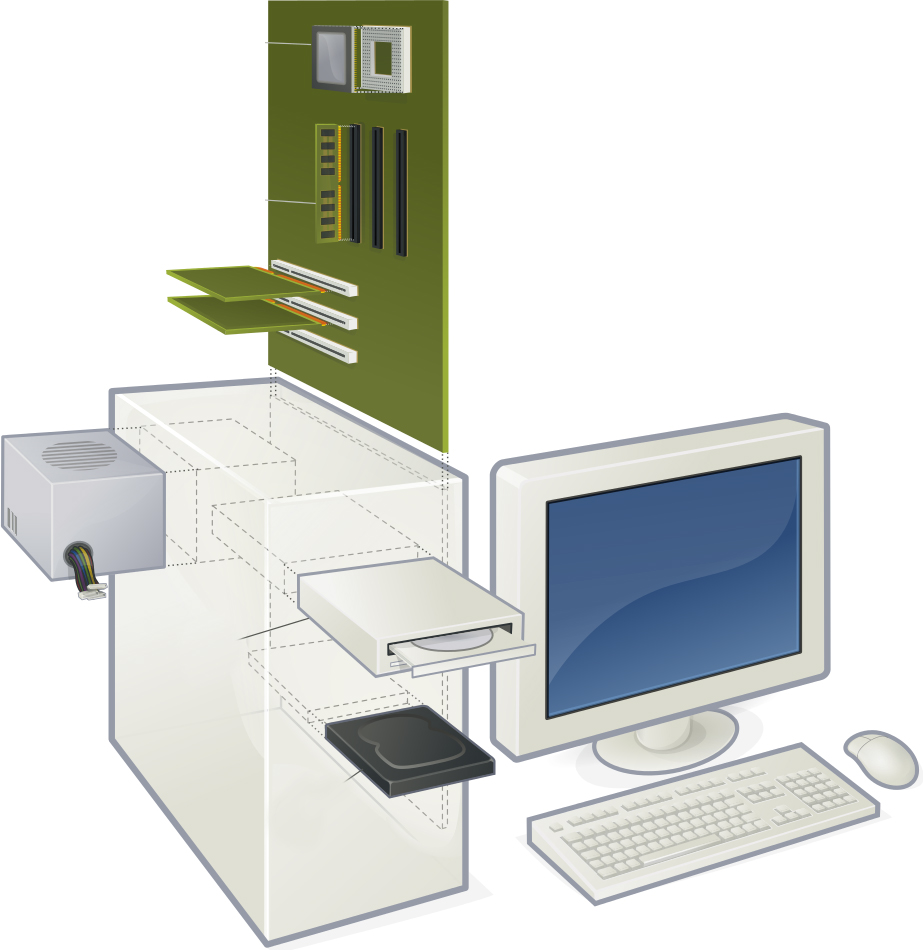
\includegraphics[width=0.3\textwidth]{./Pictures/hardware.jpg}
  \end{center}
  \rule{0.3\textwidth}{0.5pt}
  \caption{Hardware of a modern personal computer}
  \label{fig:hardware}
\end{wrapfigure}

Computer hardware is the collection of physical parts of a computer system. This includes the computer case, monitor, keyboard, and mouse. It also includes all the parts inside the computer case, such as the hard disk drive, motherboard, video card, and many others. Computer hardware is what you can physically touch.\cite{10}
\subparagraph*{Definitions}
\hfill \break
A computer system consists of two major elements: hardware and software. Computer hardware is the collection of all the parts you can physically touch. Computer software, on the other hand, is not something you can touch. Software is a set of instructions for a computer to perform specific operations. You need both hardware and software for a computer system to work.

Some hardware components are easy to recognize, such as the computer case, keyboard, and monitor. However, there are many different types of hardware components. In this lesson, you will learn how to recognize the different components and what they do.\cite{10}

%-------------------------------------------------------------------------------------------------------------------------------------------------------------------------------
% Raspberry Pi
%-------------------------------------------------------------------------------------------------------------------------------------------------------------------------------
\subsection{Raspberry Pi}
\begin{wrapfigure}{r}{0.5\textwidth}
  \begin{center}
    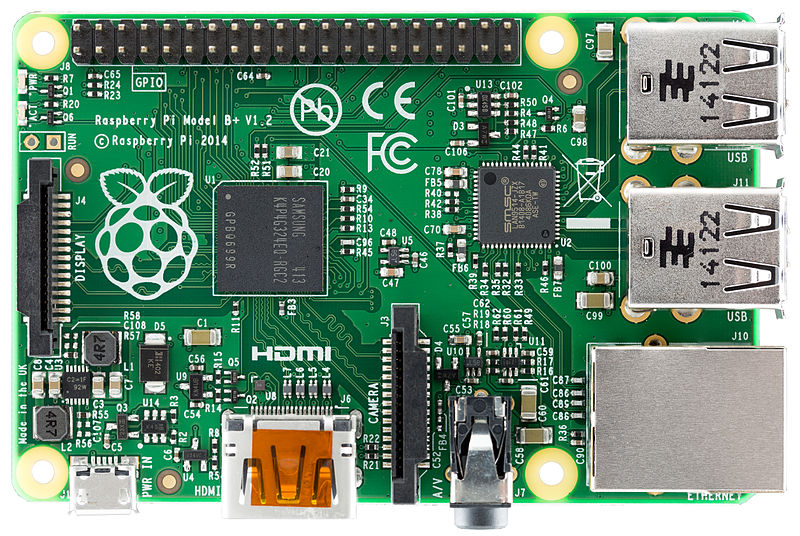
\includegraphics[width=0.5\textwidth]{./Pictures/raspberry_pi_b.jpg}
  \end{center}
  \rule{0.5\textwidth}{0.5pt}
  \caption{Raspberry Pi 1 model B+}
  \label{fig:Raspberry}
\end{wrapfigure}
\paragraph*{A brief history lesson on the Pi}
\hfill \break
Raspberry Pi\footnote{\href{https://www.raspberrypi.org/help/what-is-a-raspberry-pi/}{\texttt{https://www.raspberrypi.org/help/what-is-a-raspberry-pi/}}} (Figure \ref{fig:Raspberry}) is a series of credit card-sized single-board computers developed in the UK by the Raspberry Pi Foundation with the intention of promoting the teaching of basic computer science in schools.\cite{10}

Over the past decades, computers have gotten cheaper and cheaper, so today
you can find them not only at your desk, but also in nearly every consumer
electronics device, such as smartphones and DVD players. Still, computers
aren’t so cheap that you spontaneously buy one when shopping for your
groceries. Usually, you carefully plan your next computer purchase, because
you have to use it for a couple of years.\cite{10}

Computers like the Raspberry Pi will change the situation completely in the
near future. The Raspberry Pi or Pi, for short is a full-blown desktop PC
that costs only \$35. You can connect it directly to the Internet, and it can
display high-definition videos. Also, it runs Linux, so you don’t have to pay
for an operating system. This makes the Pi probably the first throwaway
computer in history.\cite{10}

Originally, the Raspberry Foundation \citep{2} built the Pi to teach children how to
program, so it comes as no surprise that the Pi is an excellent device for
exactly this purpose. 
On top of that, you can use the Pi for many other
exciting things. For example, you can turn it into a multimedia center, use it as a cheap but powerful web server, or play some classic games.
The Pi is also a great machine for experimenting with electronics. In contrast
to many popular microcontroller boards, such as the Arduino, the Pi runs a
full-blown operating system, and you can choose from a wide range of programming
languages to implement your projects.
With cheap and small devices like the Raspberry Pi, a new era of ubiquitous
computing has begun, and you can be part of it.\cite{10}



\paragraph*{Get to Know the Hardware}

\begin{wrapfigure}{r}{0.5\textwidth}
\vspace{15pt}
  \begin{center}
    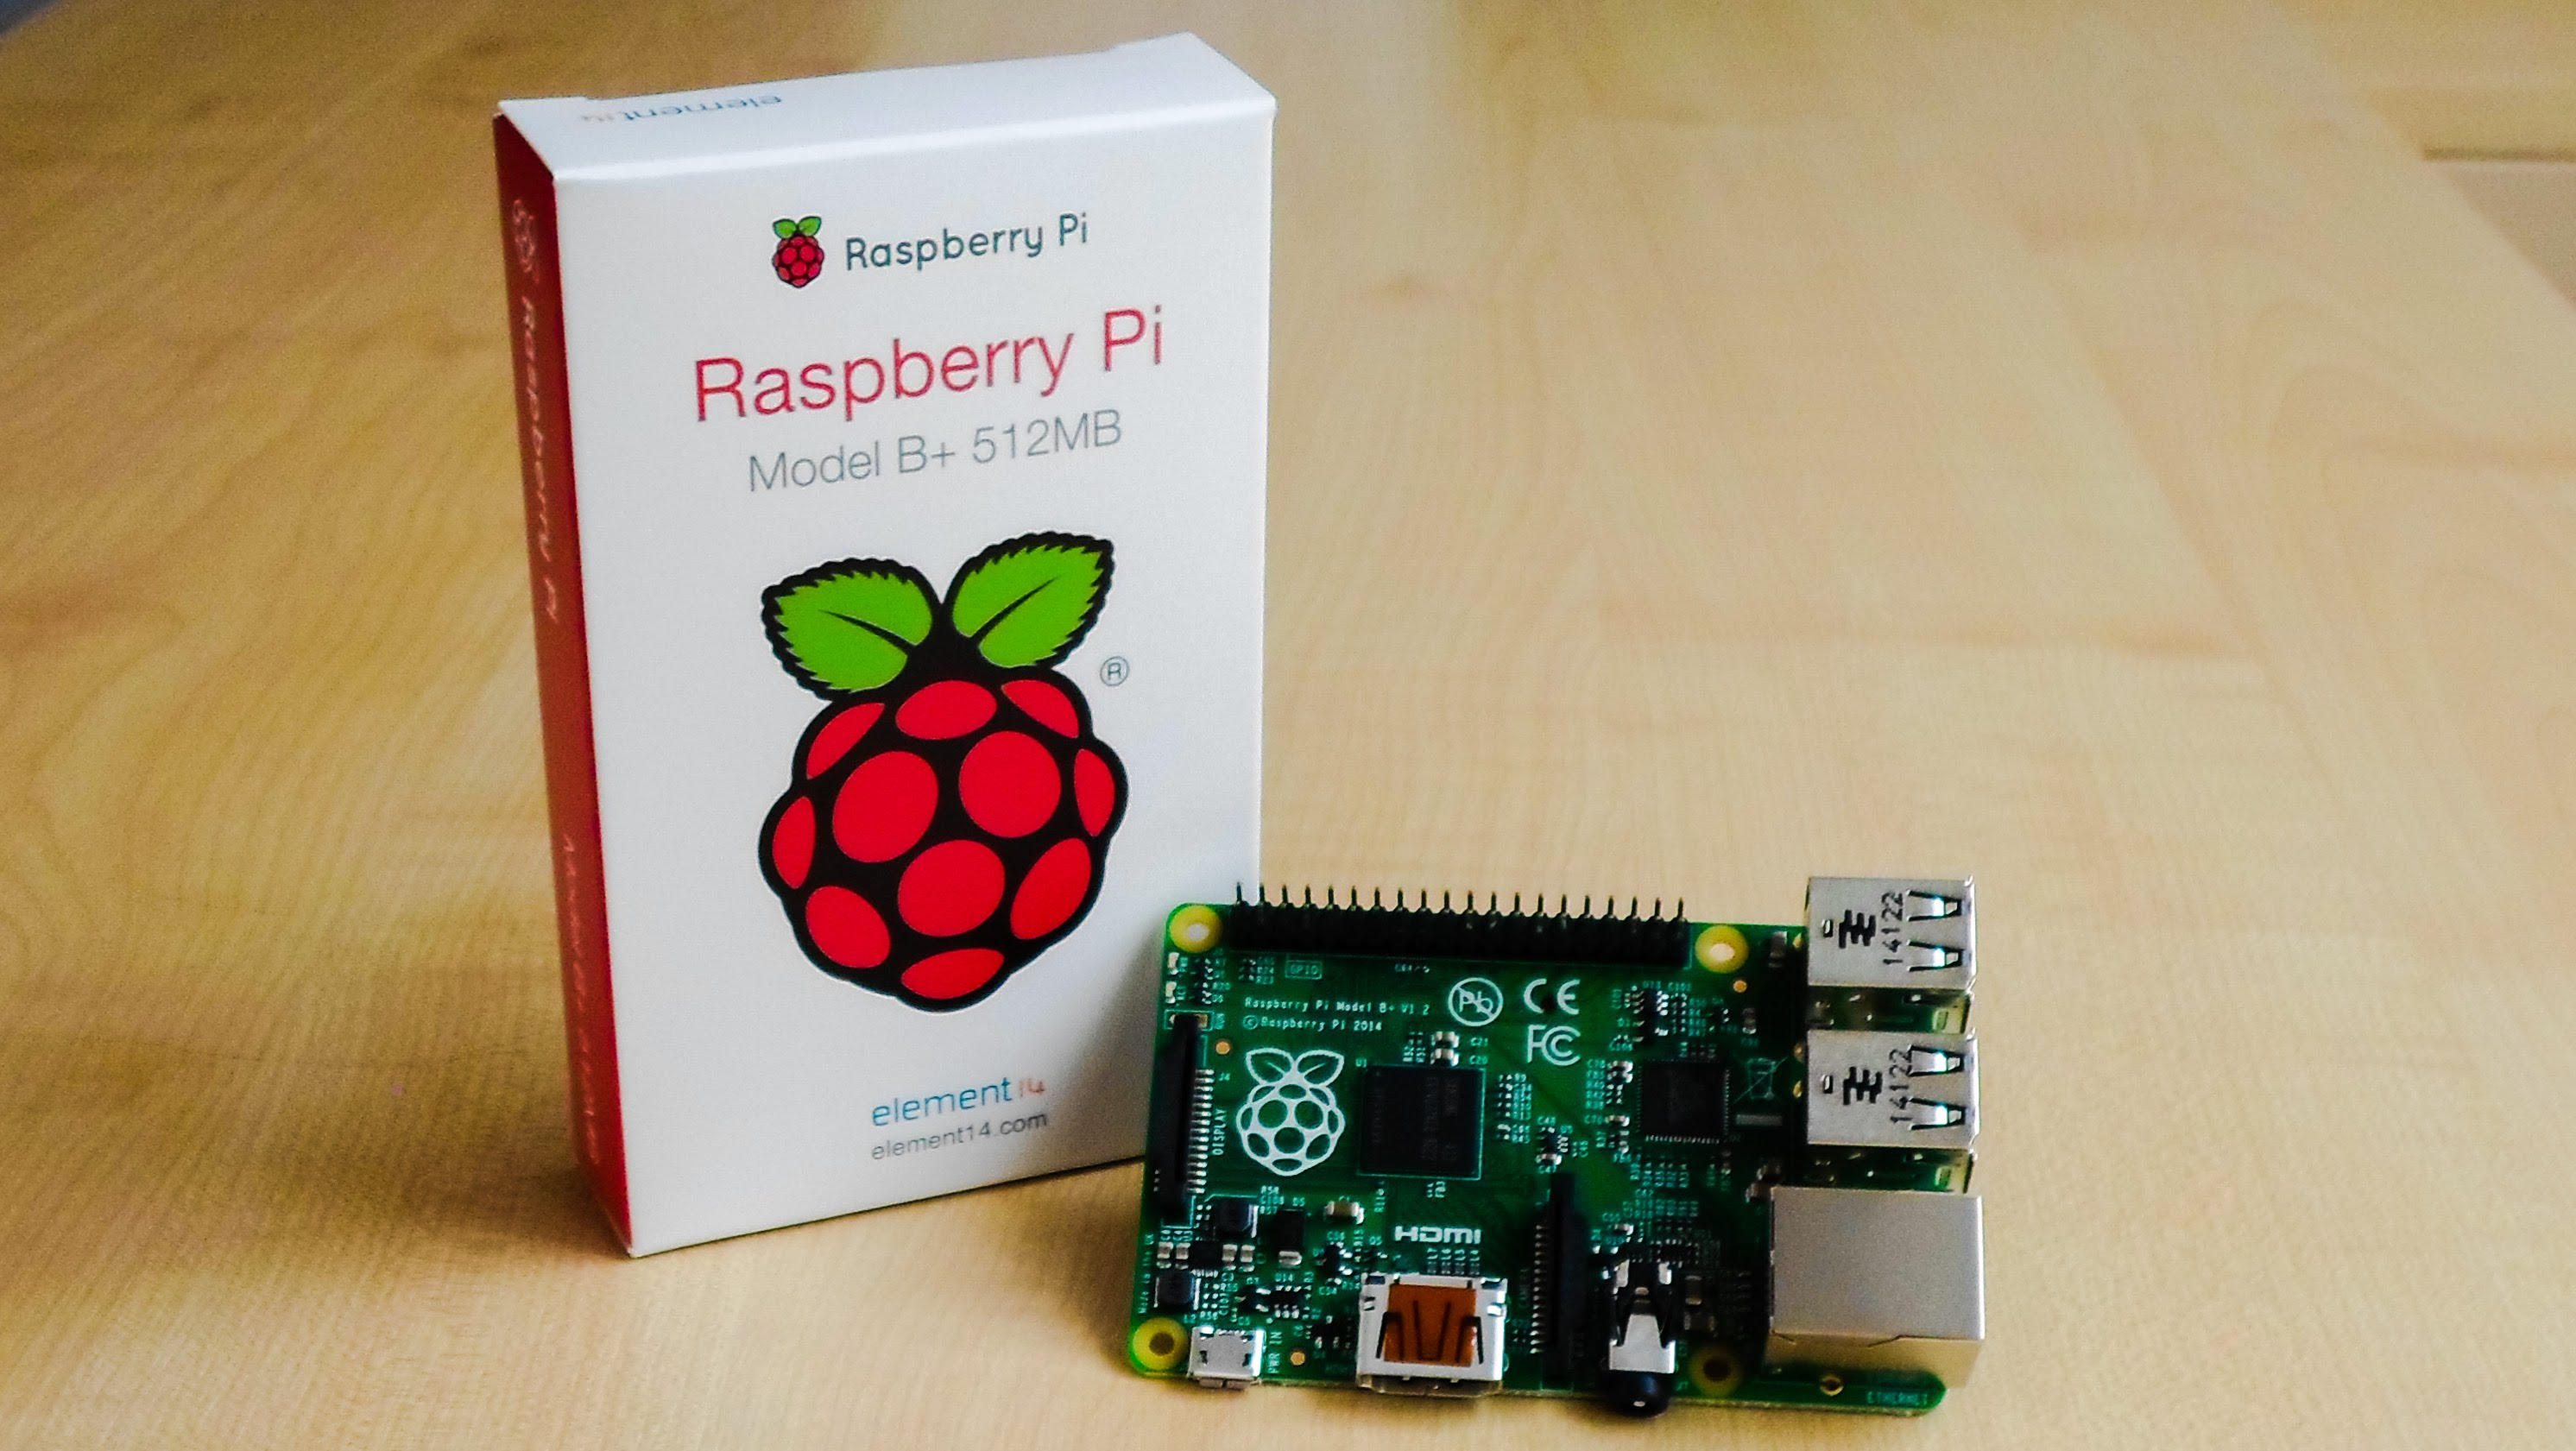
\includegraphics[width=0.5\textwidth]{./Pictures/unboxing_pi.jpg}
  \end{center}
  \rule{0.5\textwidth}{0.5pt}
  \caption{Raspberry Pi }
  \label{fig:unboxing_pi}
\end{wrapfigure}

\hfill \break
Unboxing a new Pi is exciting, but it certainly is not comparable to unboxing
a new Apple product. Usually, the Pi comes in a plain cardboard box with
one or two sheets of paper containing the usual safety hints for electronic
devices and a quick-start guide.\cite{12}

The first version of the Pi looks attractive only to real geeks (Figure \ref{fig:unboxing_pi}). It is a singleboard
computer without a case, and it’s the size of a credit card. It somewhat
resembles the innards of the many electronic devices you might have opened
when you were a child.\cite{12}

\paragraph*{What’s on the Pi}
\hfill \break
At the heart of the Pi is the Broadcom BCM2835 System-on-a-Chip—imagine all the
common hardware components of a PC baked into a small chip. The CPU is called
ARM1176JZF-S, runs at 700 MHz and belongs to the ARM11 family of the ARMv6
architecture. For graphics, the Pi sports a Broadcom VideoCore IV GPU, which is
quite powerful for such a tiny device and capable of full HD video playback. The
following figure (taken from http://www.raspberrypi.org/faqs) shows the
Raspberry Pi model:
\begin{figure}[h!]
  \centering
    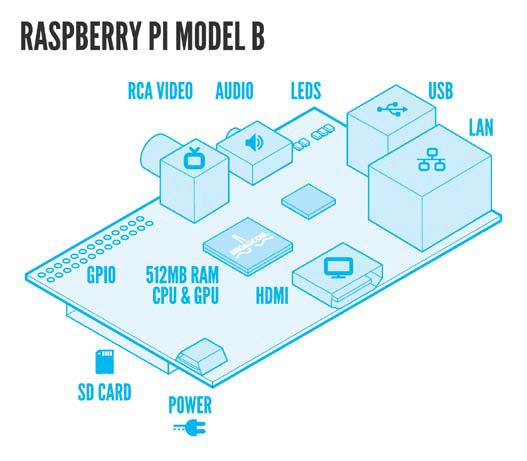
\includegraphics[width=0.5\textwidth]{./Pictures/raspberry_pi_b2.jpg}
  \rule{0.7\textwidth}{1pt}
 \caption{Raspberry Pi Model B board showing key components}
\end{figure}

\subparagraph*{GPIO}
\hfill \break
At the edge of the board we find the General Purpose Input/Output (GPIO) pins,
which, as the name implies, can be used for any kind of general tinkering and to
interface with other pieces of hardware.\cite{12}

\subparagraph*{RCA video}
\hfill \break
This jack is for composite video output, which we can use to connect the Pi to one of
those old television sets using an RCA connector cable.\cite{12}

\subparagraph*{Audio}
\hfill \break
To get sound out of the Pi, we can either get it through the HDMI cable connected
to a monitor, or from this 3.5 mm analog audio jack using headphones or
desktop speakers.\cite{12}

\subparagraph*{LEDs}
\hfill \break
Five status LEDs are used to tell us what the Pi is up to at the moment. They are
as follows:\cite{12}
\begin{itemize}
  \item The green light on top labeled OK (on the older Pi) or ACT (on the newer Pi)
will blink when the Pi is accessing data from the SD card
  \item The light below, labeled PWR, should stay solid red as long as the Pi
has power
  \item The three remaining LEDs will light up when a network cable is connected
to the Ethernet port
\end{itemize}

\subparagraph*{USB}
\hfill \break
The two USB 2.0 ports allow us to connect keyboards, mice, and most importantly
for us, Wi-Fi dongles, microphones, video cameras, and GPS receivers. We can also
expand the number of USB ports available with the help of a self-powered USB hub.\cite{12}

\subparagraph*{LAN}
\hfill \break
The Ethernet LAN port allows us to connect the Pi to a network at a maximum speed
of 100 Mbit/s. This will most commonly be a home router or a switch, but it can also
be connected directly to a PC or a laptop. A Category 5 twisted-pair cable is used for
wired network connections.\cite{12}

\subparagraph*{HDMI}
\hfill \break
The High-Definition Multimedia Interface (HDMI) connector is used to connect the
Pi to a modern TV or monitor. The cable can carry high-resolution video up to 1920 x
1200 pixels and digital sound. It also supports a feature called Consumer Electronics
Control (CEC), which allows us to use the Pi as a remote control for many common
television sets.\cite{12}

\subparagraph*{Power}
\hfill \break
The power input on the Raspberry Pi is a 5V (DC) Micro-USB Type B jack. A power
supply with a standard USB to micro-USB cable, such as a common cellphone
charger, is then connected to feed the Pi.\cite{12}

\subparagraph*{Raspbian OS}

\begin{wrapfigure}{r}{0.4\textwidth}
\vspace{-25pt}
  \begin{center}
    
\includegraphics[width=0.4\textwidth]{./Pictures/raspbian.png}
    \rule{0.4\textwidth}{1pt}
        \caption{Raspbian OS LOGO}
  \end{center}
\end{wrapfigure}
\hfill \break
Computers can't do anything useful without an operating system, and the Pi is
no exception. There is a growing collection of operating systems available for
the Pi, but we'll stick with the "officially recommended" OS—the Raspbian
GNU/Linux distribution.\cite{12}
\clearpage
%-------------------------------------------------------------------------------------------------------------------------------------------------------------------------------
% end Raspberry Pi
%-------------------------------------------------------------------------------------------------------------------------------------------------------------------------------
%-------------------------------------------------------------------------------------------------------------------------------------------------------------------------------
% Car Chassis Development Kit
%-------------------------------------------------------------------------------------------------------------------------------------------------------------------------------

\subsection{Car Chassis Development Kit} 

\begin{figure}[h!]
        \centering
        \begin{subfigure}[b]{0.5\textwidth}
                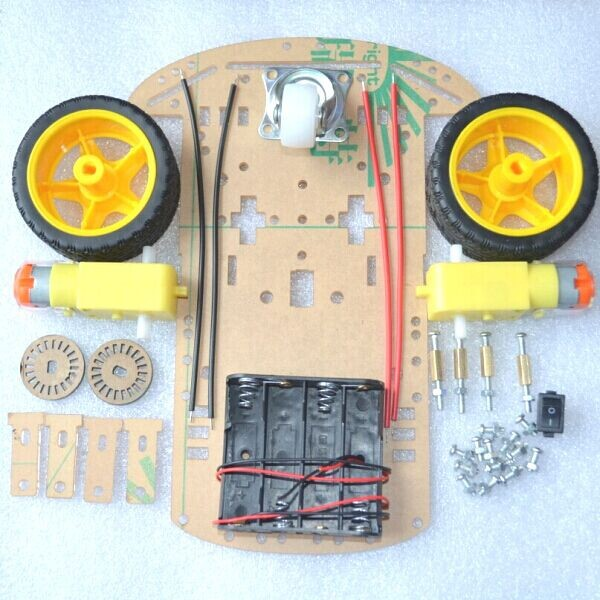
\includegraphics[width=\textwidth]{./Pictures/Car-Chassis-Kit.jpg}
        \end{subfigure}%
        ~ %add desired spacing between images, e. g. ~, \quad, \qquad, \hfill etc.
          %(or a blank line to force the subfigure onto a new line)
        \begin{subfigure}[b]{0.5\textwidth}
                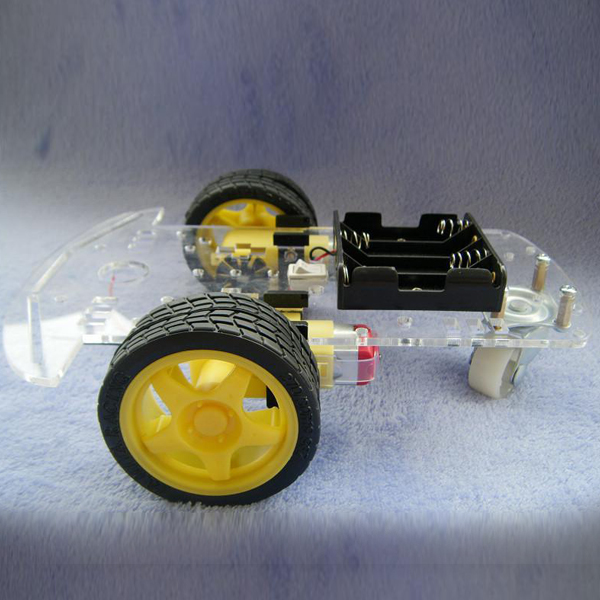
\includegraphics[width=\textwidth]{./Pictures/Car-Chassis-Kit2.jpg}
        \end{subfigure}
        \rule{1\textwidth}{1pt}
        \caption{Car Chassis Development Kit}
        \label{fig:car_chassis}
\end{figure}
\begin{figure}[h!]
        \centering
        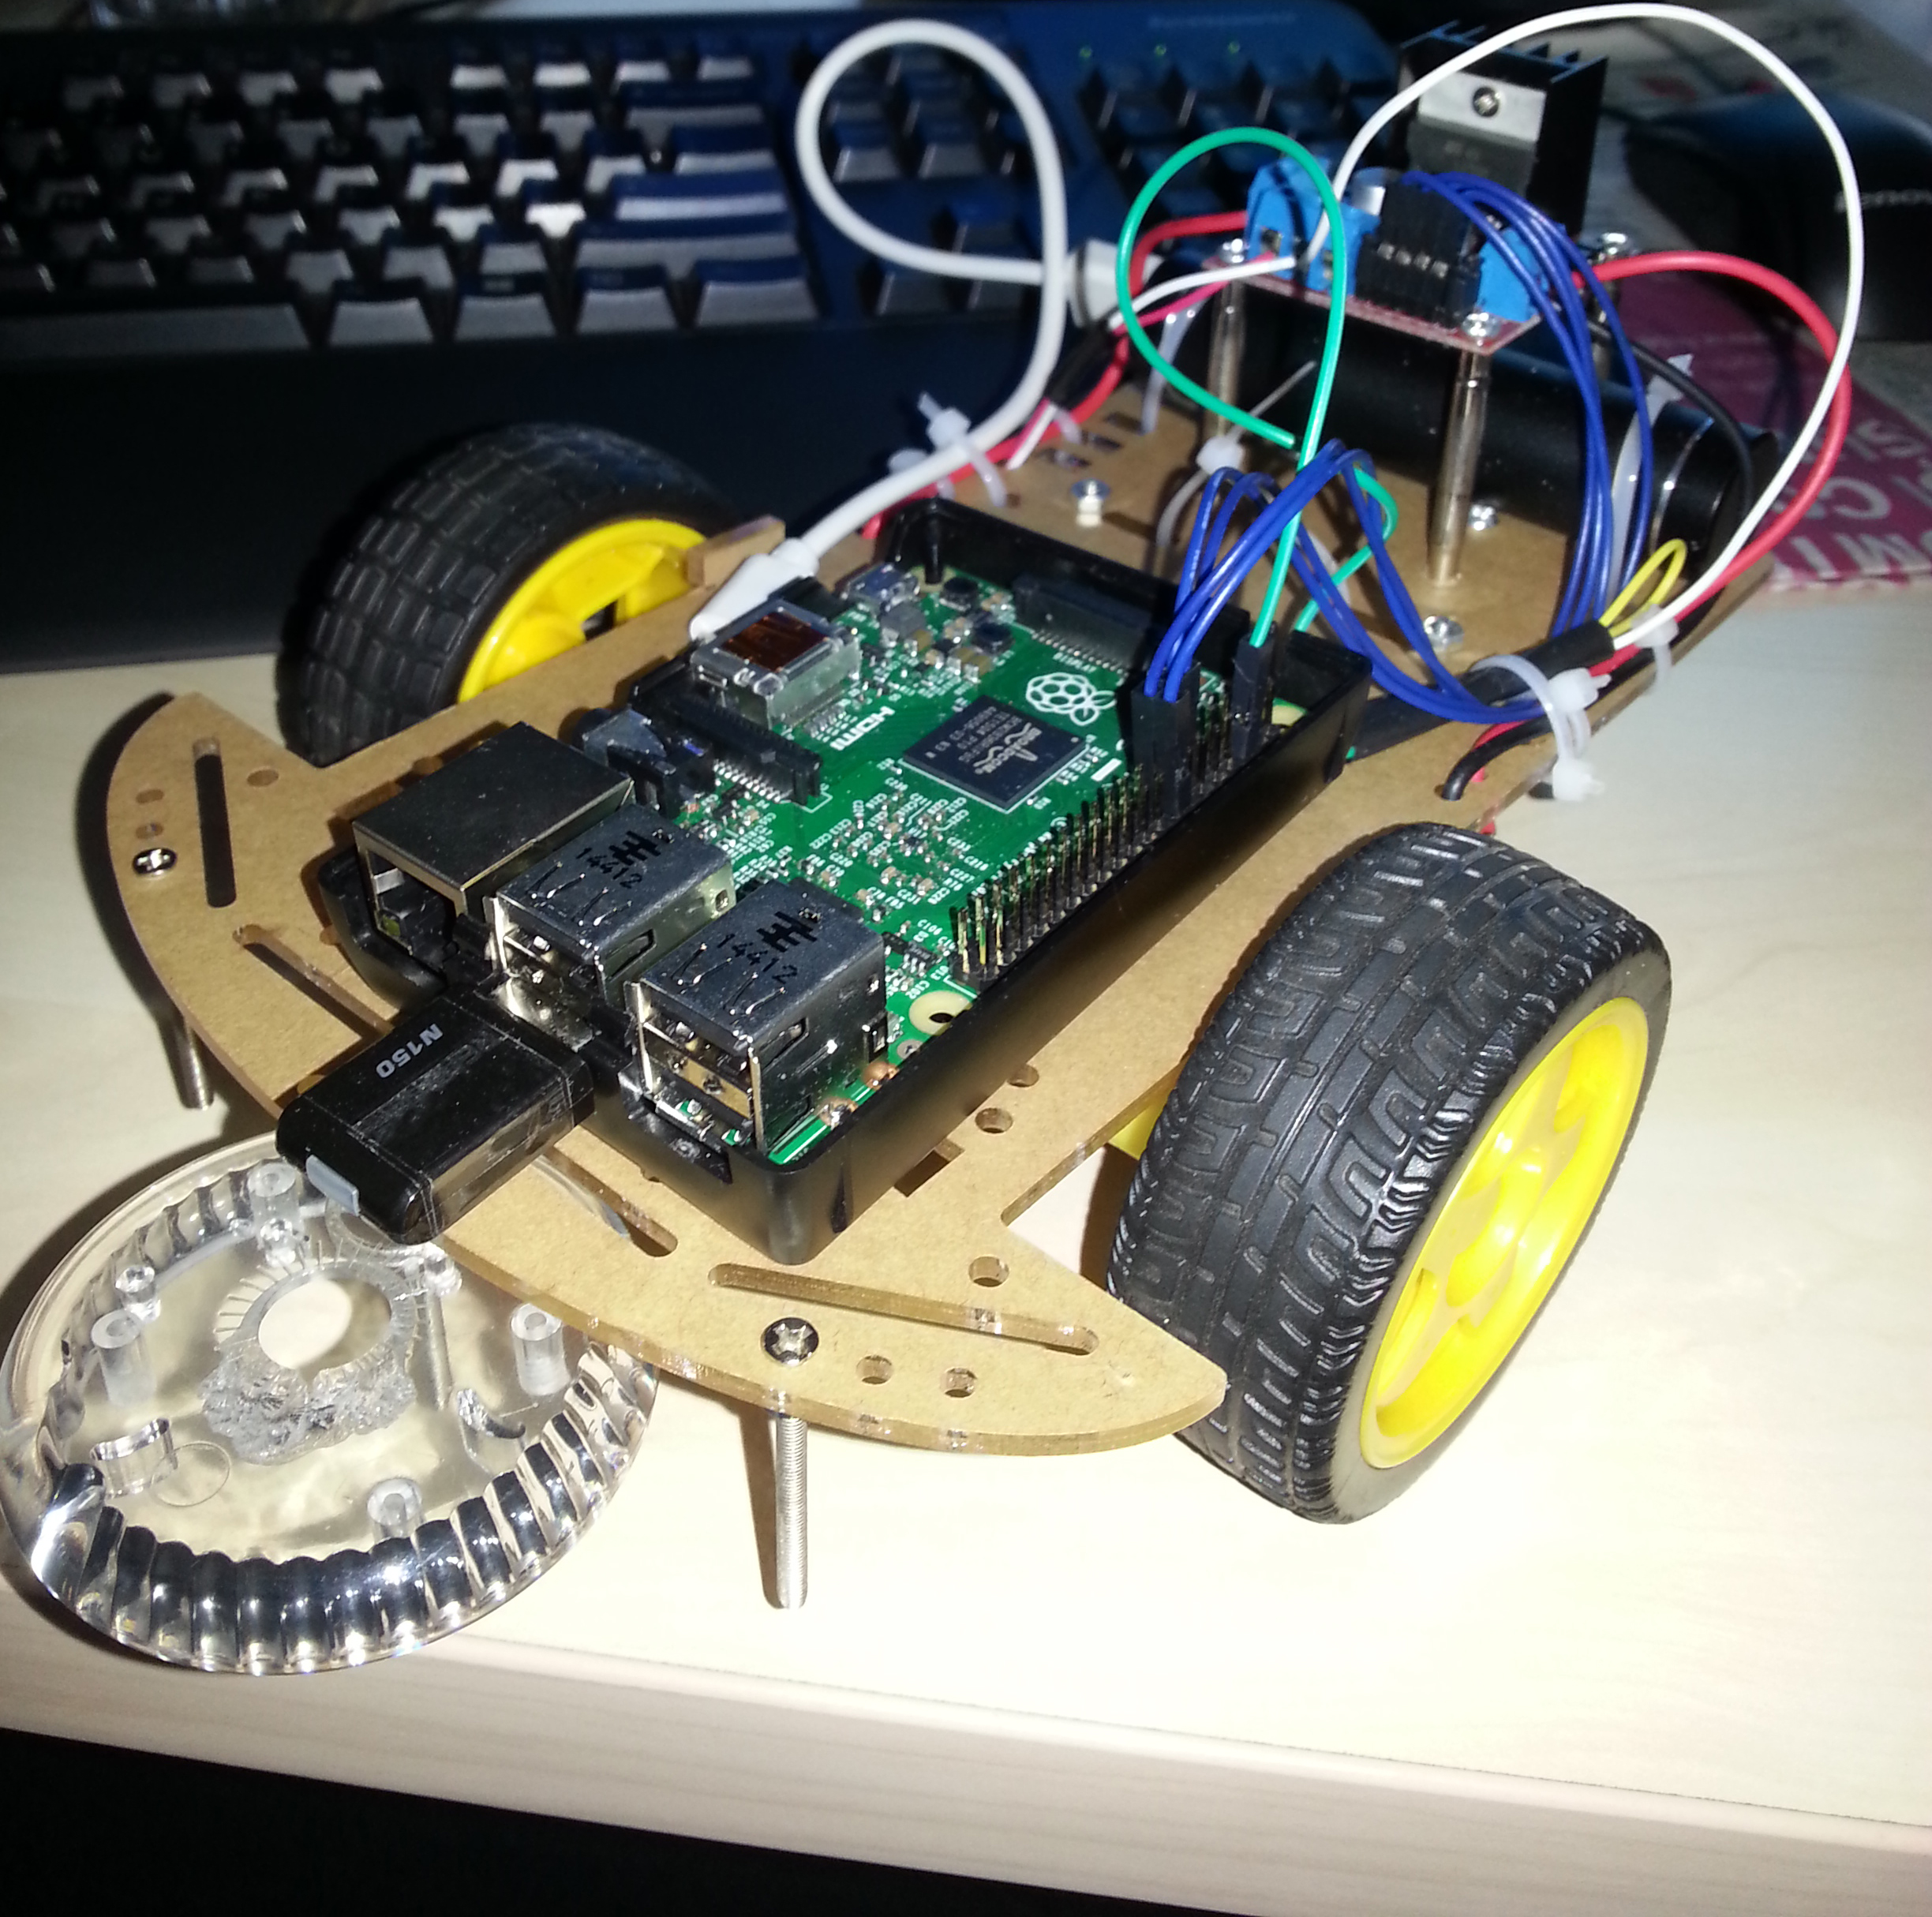
\includegraphics[width=0.5\textwidth]{./Pictures/Car-Chassis-Kit3.jpg}
		\rule{0.5\textwidth}{1pt}
        \caption{Car Chassis Development Kit}
\end{figure}
\clearpage
%-------------------------------------------------------------------------------------------------------------------------------------------------------------------------------
% end Car Chassis Development Kit
%-------------------------------------------------------------------------------------------------------------------------------------------------------------------------------
%-------------------------------------------------------------------------------------------------------------------------------------------------------------------------------
% Technologies and Programming Languages
%-------------------------------------------------------------------------------------------------------------------------------------------------------------------------------
\section{Technologies and Programming Languages}

Software is a generic term for organized collections of computer data and instructions, often broken into two major categories: system software that provides the basic non-task-specific functions of the computer, and application software which is used by users to accomplish specific tasks. \cite{14}

System software is responsible for controlling, integrating, and managing the individual hardware components of a computer system so that other software and the users of the system see it as a functional unit without having to be concerned with the low-level details such as transferring data from memory to disk, or rendering text onto a display. Generally, system software consists of an operating system and some fundamental utilities such as disk formatters, file managers, display managers, text editors, user authentication (login) and management tools, and networking and device control software. \cite{14}

Application software, on the other hand, is used to accomplish specific tasks other than just running the computer system. Application software may consist of a single program, such as an image viewer; a small collection of programs (often called a software package) that work closely together to accomplish a task, such as a spreadsheet or text processing system; a larger collection (often called a software suite) of related but independent programs and packages that have a common user interface or shared data format, such as Microsoft Office, which consists of closely integrated word processor, spreadsheet, database, etc.; or a software system, such as a database management system, which is a collection of fundamental programs that may provide some service to a variety of other independent applications. \cite{14}

Software is created with programming languages and related utilities, which may come in several of the above forms: single programs like script interpreters, packages containing a compiler, linker, and other tools; and large suites (often called Integrated Development Environments) that include editors, debuggers, and other tools for multiple languages. \cite{14}


\paragraph*{Programming Languages}
\hfill \break
There exists an enormous variety of programming languages in use today. Testimony of this fact are the 650 plus different programming languages listed in Wikipedia \footnote{\href{http://en.wikipedia.org/wiki/List_of_programming_languages}{\texttt{List of programming languages}}}. A good understanding of this great diversity is important for many reasons. First, it opens new perspectives to the computer scientist. Problems at first hard in one language might have a very easy solution in another. Thus, knowing which language to use in a given domain might decrease considerably the effort to build an application.\cite{14}


\subparagraph*{What is a Programming Languages}
\hfill \break
A programming language is an artificial language that can be used to instruct a computer to do a particular task. To be considered a general programming language, it must be computationally complete, or Turing-Complete. It is nevertheless common to regard some languages that are not computationally complete, like database query languages and other domain-specific languages as programming languages as well.\cite{14}

\subparagraph*{High-Level Versus Low-Level Programming Languages}
\hfill \break
A low-level programming language is one that is very basic and close to the machine's native language. A low-level programming language can be thought of as a building block language for software. Assembly code is the most common low-level language and requires very little translation to assemble it to machine code. (The 1's and 0's that make up binary.)

A high-level programming language is one that is closer to a level of human communication. In this method, the compiler does a lot more of the work for the programmer. The closer the language is to our everyday speech, the easier it is to worry about more complex problems. However, this can be taken too far. If a language is too much like English (or other natural languages), it can be harder to create complex programs. This is because verbose languages take more time to read, and so they can take a lot more time to understand.\cite{14}
\begin{figure}[h!]
        \centering
                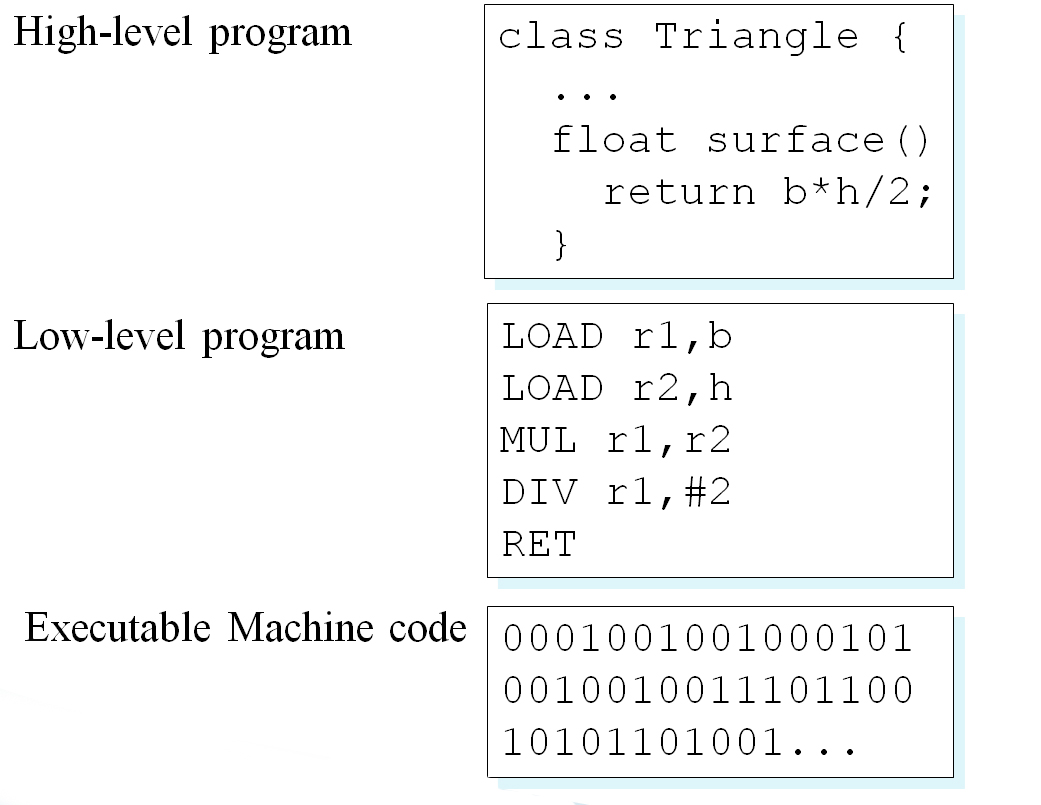
\includegraphics[width=0.7\textwidth]{./Pictures/lavels.jpg}
                  \rule{0.7\textwidth}{1pt}
        \caption{Levels of Programming Languages}
\end{figure}

Machine code is the language the computer can understand directly. Machine code consists of sequences of binary digits. It is almost never programmed in directly, but anything that is to be run on an ordinary computer must be translated to machine code first. The machine code can be different for each computer architecture. \cite{14}

Assembly language is a more human readable representation of the machine code, where the machine instructions are represented as mnemonics rather than binary digits. Assembly language has a 1:1 relationship with machine code as long as the program is not self-modifying. Before an assembly program can be run by a computer, it must be transformed to machine code. A program that does this translation is known as an assembler. In the early days of computing, assembly language was extensively used, but today it is mainly used for very time critical parts of programs, the core of operating systems, as well as in very small computers, like the chip on a smartcard. \cite{14}

Machine code and assembly language are called first and second generation programming languages respectively. A programming language that has arithmetic expressions, looping constructs, functions, and other constructs that save the programmer from dealing with the machine instructions directly is known as a third-generation programming language. \cite{14}

High-level, domain-specific programming languages were earlier often mentioned as fourth-generation languages, while expert systems were called fifth-generation programming languages. In later years this distinction has blurred, as many very high-level general purpose programming languages like Python, Haskell and Common Lisp have emerged. Expert systems are in very little use today.\cite{14}

\subparagraph*{Compilation and interpretation of computer programs}
\hfill \break
Before a program can be executed on a computer, it must be translated to machine code. Alternatively it can be simulated by another program, called an interpreter. A compiler is a program that translates a programming language, called the source programming language into another programming language, called the destination language. Usually the source language is a high level language, while the destination language is machine code. An interpreter may require that the source programming language be compiled into an intermediate form before interpretetion, called byte code. This is a more low level language, for which it is easier to write an interpreter. In the Java programming language this is a separate step, while in other cases it is performed as an integral part of the interpreter. Examples of such programming languages are Perl and Python. CommonLisp is an exception to the above: it's both interpreted and compiled.\cite{14}

\subparagraph*{Type Systems}
\hfill \break
There are two axes to type systems: Dynamic versus Static on the one side and Strong versus Weak.\cite{14}

\begin{itemize}
  \item A Strongly typed language will not allow an operation on an object if this object does not match in type. Examples are CommonLisp, Q-base and Python.
  \item A Weakly typed language will allow such operations. Examples are C and C++.
  \item TDynamic type languages bind type to value. Staticly typed languages bind it to variable.
\end{itemize}

\subsection{Web Application Back-End}
In software engineering, the terms "front end" and "back end" are distinctions which refer to the separation of concerns between a presentation layer and a data access layer respectively.
The front end is an interface between the user and the back end. The front and back ends may be distributed amongst one or more systems. \cite{14}

In software architecture, there may be many layers between the hardware and end user. Each can be spoken of as having a front end and a back end. The front is an abstraction, simplifying the underlying component by providing a user-friendly interface. \cite{14}

In software design, for example, the model-view-controller architecture provides front and back ends for the database, the user and the data processing components. The separation of software systems into front and back ends simplifies development and separates maintenance. A rule of thumb is that the front (or "client") side is any component manipulated by the user. The server-side (or "back end") code resides on the server. The confusion arises when one must make front-end edits to server-side files. Most HTML designers, for instance, don't need to be on the server when they are developing the HTML; conversely, the server-side engineers are, by definition, never on anything but a server. It takes both to ultimately make a functioning, interactive website. \cite{14}
\subsubsection{JavaScript}
JavaScript is the programming language of the Web. The overwhelming majority of
modern websites use JavaScript, and all modern web browsers—on desktops, game
consoles, tablets, and smart phones—include JavaScript interpreters, making JavaScript
the most ubiquitous programming language in history. JavaScript is part of the
triad of technologies that all Web developers must learn: HTML to specify the content
of web pages, CSS to specify the presentation of web pages, and JavaScript to specify
the behavior of web pages. This book will help you master the language.
If you are already familiar with other programming languages, it may help you to know
that JavaScript is a high-level, dynamic, untyped interpreted programming language
that is well-suited to object-oriented and functional programming styles. JavaScript
derives its syntax from Java, its first-class functions from Scheme, and its prototypebased
inheritance from Self. But you do not need to know any of those languages, or
be familiar with those terms, to use this book and learn JavaScript. \cite{1}

The name “JavaScript” is actually somewhat misleading. Except for a superficial syntactic
resemblance, JavaScript is completely different from the Java programming language.
And JavaScript has long since outgrown its scripting-language roots to become
a robust and efficient general-purpose language. The latest version of the language (see
the sidebar) defines new features for serious large-scale software development.\cite{20}

\paragraph*{JavaScript: Names and Versions}
\hfill \break
JavaScript was created at Netscape in the early days of the Web, and technically, “JavaScript”
is a trademark licensed from Sun Microsystems (now Oracle) used to describe
Netscape’s (now Mozilla’s) implementation of the language. Netscape submitted the
language for standardization to ECMA—the European Computer Manufacturer’s Association—and
because of trademark issues, the standardized version of the language
was stuck with the awkward name “ECMAScript.” For the same trademark reasons,
Microsoft’s version of the language is formally known as “JScript.” In practice, just
about everyone calls the language JavaScript. This book uses the name “ECMAScript”
only to refer to the language standard.\cite{20}


For the last decade, all web browsers have implemented version 3 of the ECMAScript
standard and there has really been no need to think about version numbers: the language
standard was stable and browser implementations of the language were, for the
most part, interoperable. Recently, an important new version of the language has been
defined as ECMAScript version 5 and, at the time of this writing, browsers are beginning
to implement it. This book covers all the new features of ECMAScript 5 as well as all
the long-standing features of ECMAScript 3. You’ll sometimes see these language versions
abbreviated as ES3 and ES5, just as you’ll sometimes see the name JavaScript
abbreviated as JS.\cite{20}


When we’re speaking of the language itself, the only version numbers that are relevant
are ECMAScript versions 3 or 5. (Version 4 of ECMAScript was under development
for years, but proved to be too ambitious and was never released.) Sometimes, however,
you’ll also see a JavaScript version number, such as JavaScript 1.5 or JavaScript 1.8.
These are Mozilla’s version numbers: version 1.5 is basically ECMAScript 3, and later
versions include nonstandard language extensions. Finally, there are
also version numbers attached to particular JavaScript interpreters or “engines.” Google
calls its JavaScript interpreter V8, for example, and at the time of this writing the
current version of the V8 engine is 3.0.\cite{20}


\subparagraph*{Why JavaScript?}
\hfill \break
JavaScript is an important language because it is the language of the web browser. Its
association with the browser makes it one of the most popular programming languages
in the world. At the same time, it is one of the most despised programming
languages in the world. The API of the browser, the Document Object Model
(DOM) is quite awful, and JavaScript is unfairly blamed. The DOM would be painful
to work with in any language. The DOM is poorly specified and inconsistently
implemented. This book touches only very lightly on the DOM. I think writing a
Good Parts book about the DOM would be extremely challenging.\cite{20}


JavaScript is most despised because it isn’t some other language. If youare good in
some other language and youhave to program in an environment that only supports
JavaScript, then youare forced to use JavaScript, and that is annoying. Most people
in that situation don’t even bother to learn JavaScript first, and then they are surprised
when JavaScript turns out to have significant differences from the some other
language they would rather be using, and that those differences matter.\cite{20}


The amazing thing about JavaScript is that it is possible to get work done with it
without knowing much about the language, or even knowing much about programming.
It is a language with enormous expressive power. It is even better when you
know what you’re doing. Programming is difficult business. It should never be
undertaken in ignorance.\cite{20}

\paragraph*{Exploring JavaScript}
\hfill \break
When learning a new programming language, it’s important to try the examples in the
book, and then modify them and try them again to test your understanding of the
language. To do that, you need a JavaScript interpreter. Fortunately, every web browser
includes a JavaScript interpreter, and if you’re reading this book, you probably already
have more than one web browser installed on your computer.\cite{20}

We’ll see later on in this chapter that you can embed JavaScript code within <script>
tags in HTML files, and when the browser loads the file, it will execute the code. Fortunately,
however, you don’t have to do that every time you want to try out simple
snippets of JavaScript code. Spurred on by the powerful and innovative Firebug extension
for Firefox (pictured in Figure \ref{fig:Firebug} and available for download from \href{http://getfirebug.com/}{http://getfirebug.com/}, today’s web browsers all include web developer tools that are indispensable for
debugging, experimenting, and learning. You can usually find these tools in the Tools
menu of the browser under names like “Developer Tools” or “Web Console.”
(Firefox 4 includes a built-in “Web Console,” but at the time of this writing, the Firebug
extension is better.) Often, you can call up a console with a keystroke like F12 or Ctrl-Shift-J.
These console tools often appear as panes at the top or bottom of the browser
window, but some allow you to open them as separate windows (as pictured in Figure
\ref{fig:Firebug}), which is often quite convenient.\cite{20}


A typical “developer tools” pane or window includes multiple tabs that allow you to
inspect things like HTML document structure, CSS styles, network requests, and so
on. One of the tabs is a “JavaScript console” that allows you to type in lines of JavaScript
code and try them out. This is a particularly easy way to play around with JavaScript,
and I recommend that you use it as you read this book.

There is a simple console API that is portably implemented by modern browsers. You
can use the function console.log() to display text on the console. This is often surprisingly
helpful while debugging, and some of the examples in this book (even in the
core language section) use console.log() to perform simple output. A similar but more
intrusive way to display output or debugging messages is by passing a string of text to
the alert() function, which displays it in a modal dialog box.\cite{20}
\begin{figure}[h!]
  \centering
    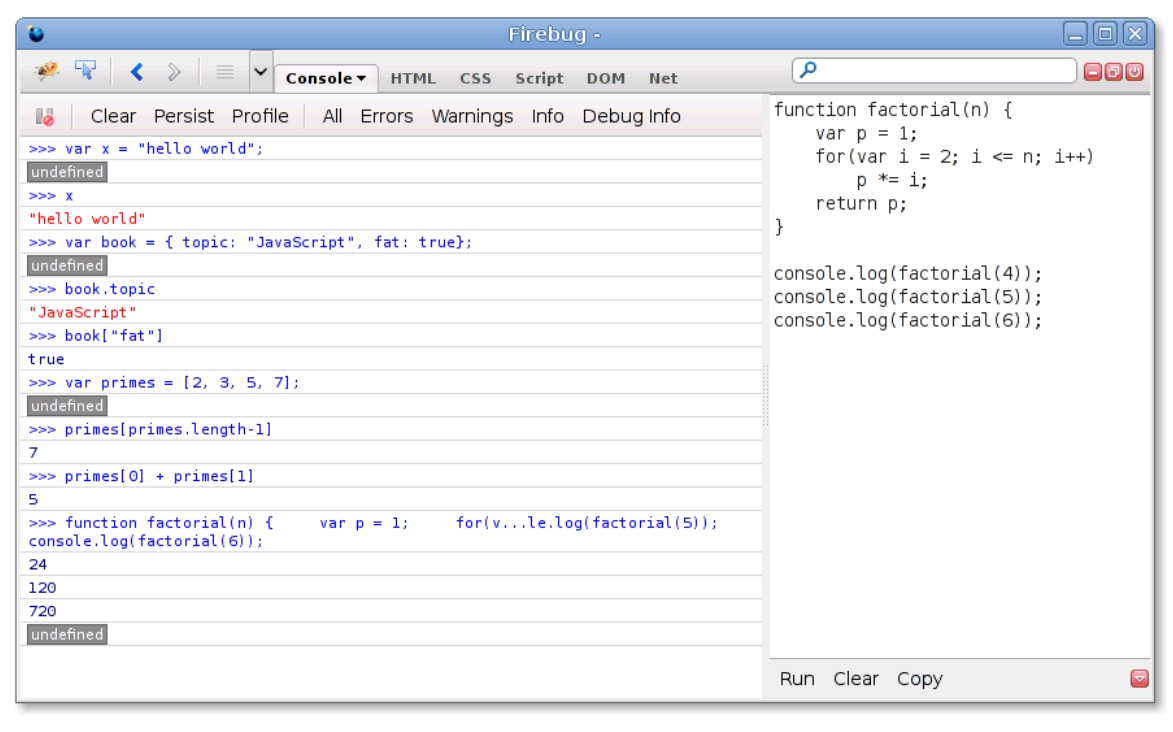
\includegraphics[width=\textwidth]{./Pictures/firebug.jpg}
  \rule{1\textwidth}{1pt}
 \caption{The Firebug debugging console for Firefox}
 \label{fig:Firebug}
\end{figure}
%-------------------------------------------------------------------------------------------------------------------------------------------------------------------------------
% end JS
%-------------------------------------------------------------------------------------------------------------------------------------------------------------------------------

\subsubsection{NodeJs}
Node.js is an open source, cross-platform runtime environment for server-side and networking applications. Node.js applications are written in JavaScript, and can be run within the Node.js runtime on OS X, Microsoft Windows, Linux, FreeBSD, NonStop and IBM i.

Node.js provides an event-driven architecture and a non-blocking I/O API that optimizes an application's throughput and scalability. These technologies are commonly used for real-time web applications.
Node.js uses the Google V8 JavaScript engine to execute code, and a large percentage of the basic modules are written in JavaScript. Node.js contains a built-in library to allow applications to act as a Web server without software such as Apache HTTP Server or IIS.\cite{17}
\clearpage



\paragraph*{Getting Started with Node.js}
\hfill \break
The definition of Node.js that is given on the Node.js website
(\href{http://nodejs.org/}{http://nodejs.org/}), is as follows:
\begin{sloppypar}
\textit{Node.js is a platform built on Chrome's JavaScript runtime for easily building
fast, scalable network applications. Node.js uses an event-driven, non-blocking I/O
model that makes it lightweight and efficient, perfect for data-intensive real-time
applications that run across distributed devices.}
\end{sloppypar}
What matters to us is, Node.js as a part of the platform, provides a scalable and
high-performance web application development framework, which allows
programming in JavaScript.\cite{18}

Many of us got introduced to JavaScript while building websites or web applications
for DOM manipulation, AJAX, and related stuff. But JavaScript is much more
than that. Just like C, Java, Python, and so on, JavaScript is also a full-fledged
programming language. In all browsers, JavaScript is executed in a virtual
machine (VM), in the context of the browser. But it can also be executed in
another context—as in the case of a Node.js backend—without the browser.\cite{18}

Node.js uses Google Chrome's JavaScript VM to execute JavaScript applications
outside the browser, on the server. Along with this runtime environment,
Node.js also provides a library of modules, which provides a framework for
building network applications. Node.js is not a web server like the Apache HTTP
server, or an application server like Tomcat; but as part of its modules library,
Node.js does provide an HTTP Server, which can be used to build web applications.\cite{18}

Apart from having JavaScript as the programming language for the applications,
one thing that sets Node.js (and most of the Node.js modules and applications)
apart from the traditional servers and applications is the asynchronous event-driven
development model, which we will see in later sections.\cite{16}

\paragraph*{The origin of Node.js}
\hfill \break
This is not the first time that JavaScript has been used for server-side programming.
Netscape launched Netscape Enterprise Server in 1996, which allowed server-side
programming in JavaScript. Since then, many servers, such as \textbf{RingoJS}
(\href{http://ringojs.org/}{http://ringojs.org/}), \textbf{Persevere} (\href{http://www.persvr.org/}{http://www.persvr.org/}), Mozilla's
Rhino-based servers, and others have tried to follow suit.\cite{16}

A major reason for these servers not being taken seriously was the pitiful performance
of the JavaScript VMs used by them. JavaScript performance in browsers was also not
very good. That was until Google launched its Chrome web browser.\cite{16}

At the time of its launch, Chrome's JavaScript VM, called V8, was almost 10-20 times
faster than any other JavaScript VM, and has since then been the fastest.\cite{16}

It was based on this VM that Ryan Dahl developed Node.js in 2008. He wanted to
build a server that would enable and empower real-time interactive web applications
like Gmail. But Node.js was not the first server he built. Ryan built Ebb, a web server
based on Ruby and C, but realized that it wasn't working as fast as he wanted it to.
This was followed by several experiments in building a number of small web servers.\cite{16}

Armed with the knowledge gained from his experiments and the study of various
platforms, he decided to develop an event-driven or asynchronous server. In the
January of 2008, he came up with the idea of building a small web server based on
JavaScript. He was inclined towards JavaScript because it was independent of the
OS and came without any I/O APIs. He quit his job and worked on Node.js for 6
months. In November 2009, he presented Node.js in JSConf, and has been working
for Joyent since then. Initially, Node.js worked only on Unix-based systems; later, it
came with support for Windows OS too.\cite{16}

\paragraph*{History}
\hfill \break
Node.js was invented in 2009 by Ryan Dahl, and other developers working at Joyent. Node.js was created and first published for Linux use in 2009. Its development and maintenance was spearheaded by Ryan Dahl and sponsored by Joyent, the firm where Dahl worked.\cite{18}

Dahl was inspired to create Node.js after seeing a file upload progress bar on Flickr. The browser did not know how much of the file had been uploaded and had to query the Web server. Dahl desired an easier way.\cite{18}

It garnered international attention after its debut at the inaugural European JSConf on November 8, 2009. Dahl presented Node.js, which combined Google's V8 JavaScript engine, an event-loop, and a low-level I/O API. The project received a standing ovation, and has since then experienced significant growth, popularity and adoption.\cite{18}

In 2011, a package manager was introduced for Node.js library, called npm. The package manager allows publishing and sharing of open-source Node.js libraries by the community, and simplifies installation, updating and uninstallation of libraries.\cite{18}

In June 2011, Microsoft partnered with Joyent to implement a native Windows version of Node.js. The first Node.js build to support Windows was released in July.\cite{18}

In January 2012, Dahl stepped aside, promoting coworker and npm creator Isaac Schlueter to manage the project.\cite{18}

In January 2014, Schlueter announced Timothy J. Fontaine would be Node.js's new project lead.\cite{18}

In December 2014, Fedor Indutny started io.js, a fork of Node.js. Due to internal conflict over Joyent's governance, io.js was created as an open governance alternative with a separate technical committee.\cite{18}

\paragraph*{Why Node.js}
\hfill \break
Node.js is a new platform and is still evolving (not even a version 1.0 has been
released yet), but even in its infancy, it is probably one of the most popular platforms
on the Web. It is already powering a large number of popular services. Let us take a
look at what makes Node.js such a tempting and popular proposition.\cite{16}

\paragraph*{JavaScript everywhere}
\hfill \break
The first and foremost advantage of Node.js is JavaScript. If you know and code in
JavaScript regularly, you already know most of Node.js; all that's left to learn can be
thought of as APIs and best practices.\cite{16}

Node.js—built over Google Chrome's V8 JavaScript engine—allows entire
applications to be written using JavaScript. We have already been writing frontends
in JavaScript; with Node.js, we write the backend as well, in the same language that
we have honed our skills on and grown to love. It saves every frontend developer
from learning one more language or relying on some other developer to expose the
RESTful APIs required by their application.\cite{16}

\paragraph*{Event-driven design}
\hfill \break
Node.js was designed around events and callbacks. As a JavaScript developer, you
would already be familiar with the concept of listening to events and using callbacks.
Node.js incorporates this philosophy in each and every aspect of the platform. Be it
in server request handling, I/O, or database interactions, everything in Node.js will
ideally be handled by a callback attached to an event by a listener.\cite{16}

This brings us to one of the most important concepts behind Node.js, that is, the event
loop. I like the fast food restaurant analogy by Dan York (http://code.danyork.com)
for explaining event loop-based systems.\cite{16}

Consider a restaurant where you go to the cashier, place your order, and wait till
your food is ready. In this case, the cashier cannot serve the other customers till you
have your order, and the queue is blocked. If the restaurant has a large inflow of
customers and needs to scale up, they will have to invest in hiring more number of
cashiers, creating more cash counters, and so on. This is similar to the traditional
multithreading model.\cite{16}

In contrast, let us see the model many other restaurants use. In this case, you go
to the cashier and place your order (which he/she hands over to the kitchen);
he/she then accepts your payment and gives you a token. You then step aside, and
the cashier moves on to the next customer. When your order is ready, the kitchen
server announces this by calling your name or flashing your token number, and you
walk up and fetch your order. This event-oriented approach optimizes the work of
the cashier and lets you wait on the side, freeing up the relevant resources to service
others until your work is done.\cite{16}

In Node.js, the server is the cashier, and all the handlers are the kitchen crew. The
server accepts a request and spins it off to a handler. It then moves on to accept other
requests. When the request is processed and the results are in place, the response is
queued on the server and sent back to the client when it reaches the front of the queue.\cite{16}

As opposed to the traditional approach of launching the threads or processes of the
server (which is similar to adding more cashiers), this method is more efficient, as the
workers launched have dedicated responsibilities. This is much lighter and cheaper
than replicating the entire server.\cite{16}

In the sections ahead, we will see that we register the handlers or the workers with
the server to handle certain requests, and all the server does is delegate the requests
to these workers.\cite{16}

The advantage of the event-driven design is that everything we design is
non-blocking. "You don't wait on me, I call you" is the mantra that relieves us from
the pain involved in waiting on a request to be fulfilled. It frees up the system
resources that would have otherwise been spent in waiting on the request, so that
they can be used for the other tasks in the queue. This allows the Node.js applications
to give a very high performance and capability of handling a very high load.\cite{16}

Node.js is a modular framework with a modern module system from the ground
up. Everything in Node.js is built as modules running in the V8 JavaScript engine.
Every functionality in the platform is provided by means of modules. This keeps
the platform lean and brings in only that what is required. Having a native module
system also helps in keeping our applications modular.\cite{16}

JavaScript has become one of the most widely-used languages in the past few years
and has a vibrant community. Node.js provides developers with a good platform
that assists them in developing end-to-end applications in JavaScript. Node.js has
also brought in many revolutionary concepts, namely, always asynchronous,
non-blocking I/O, event-oriented servers, and so on. This has resulted in a very
vibrant, large, and active community. New modules are coming up continuously,
and the community provides active support and is very helpful. Most of the popular
modules and frameworks built for Node.js generally come from the community and
are mostly open source.\cite{16}

\paragraph*{Corporate backing}
\hfill \break
Many companies have invested heavily in Node.js in the past couple of years. From
Ryan Dahl's employer, Joyent, to the creators of the Mojito framework (Internet giant
Yahoo!), many companies have built products, platforms, frameworks, and services
around Node.js. This kind of corporate commitment assures a stable future.\cite{16}

\paragraph*{How to get Node.js}
\hfill \break
Due to the popularity of Node.js, it is very easy to get it working on any operating
system. You can go to \href{http://nodejs.org/}{http://nodejs.org/} and download the appropriate
distribution for your operating system. \cite{16}

If you are using Linux, in most cases, you should be able to install Node.js using
your distribution's package manager. As this information keeps changing, I'll just
point out the location instead. You'll find the instructions for installing Node.js using
package manager here:

\textbf{\href{https://github.com/joyent/node/wiki/Installing-Node.js-via-packagemanager}{https://github.com/joyent/node/wiki/Installing-Node.js-via-packagemanager}}


If you are using Mac OS or Windows, you should know that Node.js now provides
an installer for these platforms, which is the recommended installation approach.
You can also install using the source. Instead of repeating that process here, which
is again subject to change, I'll suggest that you follow the official installation
instructions on the Node.js wiki, on GitHub (https://github.com/joyent/node/
wiki/Installation).

\paragraph*{Node.js package manager (npm)}
\hfill \break
If you installed Node.js using the installer from the Node.js website, you will already
have npm installed.

Also, if you followed the instructions to build from the source, you will probably
have installed npm. If that is a yes, very good! If no, please do so now. For this,
I recommend that you follow the instructions mentioned in the npm installation
documentation (https://github.com/isaacs/npm/).\cite{16}

You can check if you have npm installed by typing the following command:

\begin{lstlisting}
$ npm -v
\end{lstlisting}

This should display the version of npm installed.

For those who are wondering what npm is and why you would need a package
manager for Node.js, npm is just what its name says; it provides an infrastructure
in Node.js to distribute and manage packages. As I said earlier, Node.js is very
modular. Node.js apps are built using many modules and third-party packages
because npm provides an easy way of adding and managing third-party
dependencies for our applications. We will see more on its use in a while.\cite{16}

\paragraph*{Hello World with Node.js}
\hfill \break
Here, the obligatory Hello World example uses Node.js. Write the following line in a
file called \textit{helloworld.js} and save it:
\begin{lstlisting}
console.log("Hello World");
\end{lstlisting}
And now to run it, execute the following command:
\begin{lstlisting}
node helloworld.js
\end{lstlisting}
This should print \textbf{Hello World} on the console. All the JavaScript developers will
immediately recognize that these are the steps we follow to print anything on the
console while developing a web application.

What happens is that Node.js loads the JavaScript file in the JavaScript VM, provides
an environment for its execution, and the VM interprets the script. When it gets
console.log, it checks the environment for the console, which in this case is STDOUT,
and writes Hello World to it.\cite{21}
%-------------------------------------------------------------------------------------------------------------------------------------------------------------------------------
% END NODEJS
%-------------------------------------------------------------------------------------------------------------------------------------------------------------------------------


\subsubsection{ExpressJs}
Express.js is a Node.js web application framework, designed for building single-page, multi-page, and hybrid web applications.
Express is a minimal and flexible Node.js web application framework that provides a robust set of features for web and mobile applications.\cite{16}
\paragraph*{Starting with Express.js}
\hfill \break
Express.js is a web framework based on the core Node.js http module and Connect components. Those components are called middleware. They are the cornerstone of the framework’s philosophy, which is configuration over convention. Some developers familiar with Ruby compare Express.js to Sinatra, which has a very different approach from the Ruby on Rails framework that favors convention over configuration. In other words, developers are free to pick whatever libraries they need for a particular project. This approach provides them with flexibility and the
capability to highly customize their projects.\cite{15}

If you have written any serious apps using only the core Node.js modules, you most likely found yourself reinventing the wheel by constantly writing the same code for similar tasks, such as:
\begin{itemize}
  \item Parsing HTTP request bodies
  \item Parsing cookies
  \item Managing sessions
  \item Organizing routes with a chain of if conditions based on URL paths and HTTP methods of the
requests
  \item Determining proper response headers based on data types
  \item Handling errors
  \item Extracting URL parameter (e.g., /messages/3233)
\end{itemize}
\cite{15}
%-------------------------------------------------------------------------------------------------------------------------------------------------------------------------------
% END EXPRESSJS
%-------------------------------------------------------------------------------------------------------------------------------------------------------------------------------
\subsubsection{Socket.io}
Socket.IO enables real-time bidirectional event-based communication.
It works on every platform, browser or device, focusing equally on reliability and speed.\cite{15}
\paragraph*{Going Real Time on the Web}
\hfill \break
The Arab Spring revolution was sparked and fuelled through social media sites like
Facebook and Twitter. Over the next few days, social media went from being just
a means of interacting with family and friends to a weapon that empowered the
people and brought about a significant change in the world. Everyone noticed the
power of the people and people noticed what social networks were capable of. At
the heart of it all was the technology that made all this possible, the technology that
removed all the barriers to communication and spread the word faster than wildfire.
This is the power of real-time web!\cite{15}

\subparagraph*{What is real-time web?}
\hfill \break
On the Web, we have been habituated to sites and applications where we click on a
link or a button, or change some input and perform some action, and it causes some
change in the page. But if we leave our twitter page open for a while, we get alerts
when we receive new tweets, even without performing any action (shown in the next
screenshot). This is what we mean in general when we say "real-time web".
Wikipedia introduces real-time web in these words:\cite{15}

\textit{The real-time web is a set of technologies and practices that enable users to receive
information as soon as it is published by its authors, rather than requiring that they
or their software check a source periodically for updates.
}
This "set of technologies" is one of the hottest trends on the Web. Over the
next few pages, we will get familiar with these technologies and see their use
in various applications.\cite{15}

\subparagraph*{A bit of history}
\hfill \break
To understand and fully appreciate any concept, it is important to know where it
came from and how it evolved.

Real-time web is not a new thing; one of the first attempts at making web real-time
was the usage of Java applets. Many will remember chatting in Yahoo! chat rooms or
playing chess, way back in the late '90s. Then came Flash and ActiveX plugins. This
was not only for "fun" (for the consumer section), but also for use in the enterprise
market. I worked for a BPM (Business Process Management) company in the early
stages of my career, where they had built an ActiveX plugin for powering their
dashboards and updating process information in real time. So why is it important
now? Because the way in which real-time functionality is implemented and the cost
involved in doing so has changed. From being a fancy feature in an application,
it has become a necessity—a user demand. From being a hacked-in or technically
challenging piece of the application, it is on its way to becoming a ratified standard
in the form of WebSockets and Server-Sent Events (SSE). How did we get from static
web to here?\cite{15}

The Web (and web applications), as we all know, is built over the HTTP protocol.
HTTP is a request-response system, where the client sends a request for information
to the server and the server responds with the requested information. In most
cases, this information is the HTML or related information, like XML or JSON, to
be rendered by the browser. This HTTP browser-server interaction is shown in the
following figure:

\begin{figure}[h!]
  \centering
    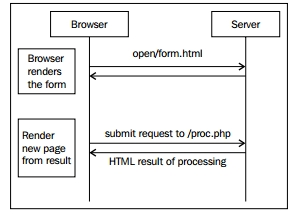
\includegraphics[width=0.5\textwidth]{./Pictures/http.jpg}
  \rule{0.5\textwidth}{1pt}
    \caption{HTTP browser-server interaction}
\end{figure}

In 1995, Sun and Netscape announced a partnership that saw Netscape bundle
Sun's brand new Java runtime with its browser. This was the beginning of highly
interactive web. Although they have since earned themselves a very bad reputation,
applets were the pioneers in the field of real-time web. In the early days of real-time
web, we saw applets being used everywhere, for chat, games, and even for banners.
In the same year, Netscape came up with a scripting language called JavaScript
(originally LiveScript), and another small company called FutureWave Software
started working on an animation software called FutureSplash Animator. Later,
both of them became the cause of Java applets almost disappearing from the Web.\cite{15}

FutureWave was acquired by Macromedia in 1996 and they renamed FutureSplash
Animator to Flash. Flash, as we all know, went on to rule the Web as the most widely
available platform for creating animations, games, video players, and everything
interactive, for the major part of the next decade.\cite{15}

In 1999, Microsoft used its iframe technology and JavaScript to update news and
stock quotes on Internet Explorer's default home page (http://home.microsoft.
com). In the same year, they released a proprietary ActiveX extension for IE, called
XMLHTTP. This was the era when XML was the "in" thing and everyone wanted to
use XML for anything they were doing. This XMLHTTP component was originally
meant to load XML data in the page asynchronously, using JavaScript. It was soon
adopted by Mozilla, Safari, and Opera, as XMLHttpRequest (or XHR, for short).
But it was with the launch of Gmail (by Google) that the term AJAX (Asynchronous
JavaScript and XML)—coined by Jesse James Garrett in an article titled \textit{Ajax: A
New Approach to Web Applications}—became the buzzword in web development. The
following figure shows an AJAX Request:
\begin{figure}[h!]
  \centering
    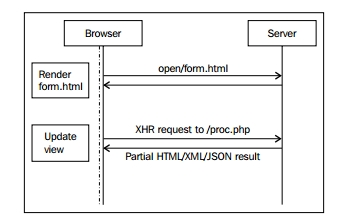
\includegraphics[width=0.5\textwidth]{./Pictures/ajax.jpg}
  \rule{0.5\textwidth}{1pt}
  \caption{AJAX Request}
\end{figure}
Gmail also shed light on the advantages of live updates to web pages and opened the
floodgates to various hacks built over AJAX to push data from a server (or at least,
giving the illusion of doing so).\cite{15}

Collectively, these technologies were referred to as Comet-a term introduced by Alex
Russell on his blog in 2006. Comet was a play on the word Ajax, both being popular
household cleaners in the US. Comet was not one single approach. It introduced
multiple mechanisms to give the feeling of data being pushed from the server to the
client. These included Hidden iframe, XHR polling, XHR long polling, and Script tag
long polling (or, JSONP long polling).\cite{15}

Let us understand how these work, as they continue to remain the most commonly
available mechanisms across all modern browsers.

The first and the easiest to implement is XHR polling, in which the browser keeps
polling for data periodically, and the server keeps responding with an empty
response unless it has data to send back to the browser. Following an event, such
as receiving a mail, or creating/updating a record in the database, the server
responds to the next polling request with new data. The following figure depicts
this mechanism:
\begin{figure}[h!]
  \centering
    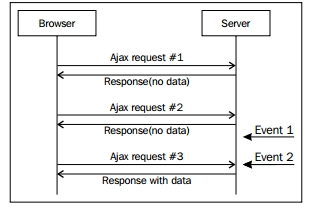
\includegraphics[width=0.5\textwidth]{./Pictures/xhr.jpg}
  \rule{0.5\textwidth}{1pt}
  \caption{XHR polling}
\end{figure}
As you can see, there is a problem with this. The browser has to keep making
requests to the server even when there is no data. This causes the server to get and
process data even when there is nothing to deliver.\cite{15}

One of the solutions to this is to modify the server to piggyback the actual client
requests by not only sending the data requested by the client, but also appending
additional data that the server has, to send to the browser. The client needs to be
modified to understand and act upon the additional incoming data. The HTTP
piggybacking process is shown in the following figure:
\begin{figure}[h!]
  \centering
    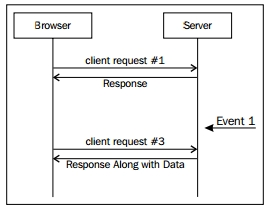
\includegraphics[width=0.5\textwidth]{./Pictures/http_2.jpg}
  \rule{0.5\textwidth}{1pt}
  \caption{HTTP piggybacking}
\end{figure}

As the new data is only sent when there is a client action, it causes delays in the
data reaching the browser. The solution to receiving events quickly while avoiding
frequent server queries is long polling.\cite{15}

In long polling, when the browser sends a request to the server, the server won't
respond immediately if it doesn't have data to respond with, and will suspend the
request. Once the event occurs, the server closes the suspended request by sending
over a response to the client. As soon as the client receives the response, it sends a
new request:
\begin{figure}[h!]
  \centering
    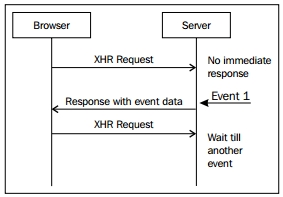
\includegraphics[width=0.5\textwidth]{./Pictures/long_poling.jpg}
  \rule{0.5\textwidth}{1pt}
  \caption{Long Polling}
\end{figure}
There are various ways in which long polling is implemented, such as forever iframe,
multipart XHR, script tags with JSONP, and long-living XHR.\cite{15}

Though all these techniques work, these are hacks, bending HTTP and XHR to be
able to do duplex communication, which is not what they are meant for.
With the rapid evolution of the web browsers lead by Firefox and then Chrome, the
long-due upgrade to HTML, called HTML5, is being widely adopted. In HTML5,
there are two new methods for pushing data from the server to the client. One is
Server-Sent Events (SSE) and the other is the full duplex WebSockets.\cite{15}

Server-Sent Events attempts to standardize Comet-like communication across
browsers. In this approach, there is a JavaScript API to create an event source, that is,
a stream over which the server can send events. This is a unidirectional protocol. We
will still be using the good old XHR. This is a good approach when you don't need
full duplex communication; just push updates from the server to client.\cite{15}

The other specification which goes on to implement a full duplex communication
protocol for the web applications is WebSockets. In WebSockets, the client initiates
a socket connection with the server, which supports this protocol as well. The server
and client will send and receive data on this socket connection.\cite{15}
\subsubsection{NoSQL}
\subparagraph*{Defining NoSQL}
\hfill \break
\textbf{According to Wikipedia:}
\textit{In computing, NoSQL (mostly interpreted as "not only SQL") is a broad
class of database management systems identified by its non-adherence to the
widely used relational database management system model; that is, NoSQL
databases are not primarily built on tables, and as a result, generally do not
use SQL for data manipulation.}\cite{8}


The NoSQL movement began in the early years of the 21st century when the world
started its deep focus on creating web-scale database. By web-scale, I mean scale to
cater to hundreds of millions of users and now growing to billions of connected
devices including but not limited to mobiles, smartphones, internet TV, in-car
devices, and many more.\cite{8}

Although Wikipedia treats it as "not only SQL", NoSQL originally started off as a
simple combination of two words—No and SQL—clearly and completely visible in
the new term. No acronym. What it literally means is, "I do not want to use SQL".
To elaborate, "I want to access database without using any SQL syntax". Why? We
shall explore the in a while.\cite{8}

Whatever be the root phrase, NoSQL today is the term used to address to the class
of databases that do not follow \textbf{relational database management system (RDBMS)}
principles, specifically being that of ACID nature, and are specifically designed to
handle the speed and scale of the likes of Google, Facebook, Yahoo, Twitter, and
many more.

\subparagraph*{History}
\hfill \break
Before we take a deep dive into it, let us set our context right by exploring some key
landmarks in history that led to the birth of NoSQL.\cite{8}

From Inktomi, probably the first true search engine, to Google, the present
world leader, the computer scientists have well recognized the limitations of the
traditional and widely used RDBMS specifically related to the issues of scalability,
parallelization, and cost, also noting that the data set is minimally cross-referenced
as compared to the chunked, transactional data, which is mostly fed to RDBMS.\cite{8}

Specifically, if we just take the case of Google that gets billions of requests a month
across applications that may be totally unrelated in what they do but related in how
they deliver, the problem of scalability is to be solved at each layer—right from data
access to final delivery. Google, therefore, had to work innovatively and gave birth
to a new computing ecosystem comprising of:
\begin{itemize}
  \item \textbf{GFS}: Distributed filesystem
  \item \textbf{Chubby}: Distributed coordination system
  \item \textbf{MapReduce}: Parallel execution system
  \item \textbf{Big Data}: Column oriented databas
\end{itemize}
%-------------------------------------------------------------------------------------------------------------------------------------------------------------------------------
% END SOCKET.IO
%-------------------------------------------------------------------------------------------------------------------------------------------------------------------------------
\subsection{Web Application Front-End} 
Front end development is the development of those elements of a website that the customer sees and interacts with directly. It is a combination of programming skills (knowing which program to choose) and aesthetics (understanding element arrangements on the screen, the color and font choices). The challenges associated with front end developers is that the tools and techniques used to create the front end of a website change constantly and so the developer needs to constantly be aware of how the field is developing.
The objective of designing a site is to ensure that when the users open up the site they see the information in a format that is easy to read and relevant. This is further complicated by the fact that users now use a large variety of devices with varying screen sizes and resolutions thus forcing the designer to take into consideration these aspects when designing the site. They need to ensure that their site comes up correctly in different browsers (cross-browser), different operating systems (cross-platform) and different devices (cross-device), which needs careful planning on the site of the developer.\cite{16}
\subsubsection{HTML (HyperText Markup Language)}
HyperText Markup Language, commonly referred to as HTML, is the standard markup language used to create web pages. It is written in the form of HTML elements consisting of tags enclosed in angle brackets (like <html>). HTML tags most commonly come in pairs like <h1> and </h1>, although some represent empty elements and so are unpaired, for example <img>. The first tag in such a pair is the start tag, and the second is the end tag (they are also called opening tags and closing tags).
Web browsers can read HTML files and render them into visible or audible web pages. Browsers do not display the HTML tags and scripts, but use them to interpret the content of the page. HTML describes the structure of a website semantically along with cues for presentation, making it a markup language, rather than a programming language.
HTML elements form the building blocks of all websites. HTML allows images and objects to be embedded and can be used to create interactive forms. It provides a means to create structured documents by denoting structural semantics for text such as headings, paragraphs, lists, links, quotes and other items. It can embed scripts written in languages such as JavaScript which affect the behavior of HTML web pages.
Web browsers can also refer to Cascading Style Sheets (CSS) to define the look and layout of text and other material. The World Wide Web Consortium (W3C), maintainer of both the HTML and the CSS standards, has encouraged the use of CSS over explicit presentational HTML since 1999.\cite{2}
\subparagraph*{A Brief History of the Internet and the World Wide Web}
\hfill \break
devices are connected to it. However, the Web and its underlying Internet infrastructure had a
very different childhood that betrays the consumer and commercial base it has today.
The Internet has its roots in the U.S. Department of Defense Advanced Research Project Agency
(ARPA) project begun in or around 1960. Among the project’s goals was the ability to network
computers quickly and across great distances. The network was to be designed to be almost
fail-safe, enabling connected computers to continue communicating even if assorted routes
between them were to fail.\cite{2}

In 1969, the ARPANet was born, connecting several key universities. The network continued
to grow, with more and more universities coming online. One of the goals of the initial
project — robust, nearly fail-safe performance — was realized via the Internet Protocol (IP).
This protocol enabled communication packets to find various routes to a destination in case one
or more of the routes became unstable. This communication protocol became the backbone of
today’s Internet, and is how the Internet got its name.\cite{2}

The Transmission Control Protocol was joined with the IP to provide a robust transmission suite,
a marriage of two protocols to offer more flexibility and the ability to create better communications
applications for the Internet.\cite{2}

In the 1980s, the Internet went through several transitions. Although it was highly populated by
educational institutions, the U.S. military hadn’t forgotten its original project. Other government
agencies also took notice and joined the crowd online; and the military decided to create its own
network, MILNET, lessening the load slightly.\cite{2}

By 1992, the Internet was far and away the most popular network in the world. During this
time, Tim Berners-Lee, a British software engineer and computer scientist, created HyperText
Markup Language to create documents, a protocol — HyperText Transfer Protocol (HTTP) — to send such documents, and the first browser editor, called the World Wide Web. The ‘‘Web’’ soon
came to the attention of the National Center for Supercomputing Applications (NCSA), where a
programming team decided to create a better browser. Thus was Mosaic born, the first browser
to support a high degree of multimedia. Mosaic helped usher in the crop of modern browsers we
use today.\cite{2}

As the Web continued to be adopted outside of the government and educational sectors, it
became more consumer-savvy. Many companies began using the Web infrastructure for marketing
and support purposes, while many Web developers began to target a wider, nontechnical,
audience.
By the early 2000s, the Web was accessible by almost any network-connected computer, many
electronic devices, and some unlikely consumer devices such as automobiles. Each of these connected
devices uses the same type of connection, the same languages to define documents, and
the same protocols to send the information.\cite{2}

As more and more nontechnical users began using the Web, web ‘‘pages’’ began to look more
like high-quality printed documents — resembling newspapers, brochures, magazines, and the
like. This movement in content signaled how far the Web had come from its inception — from
technical, text-only pages to full-color, heavily designed documents.\cite{2}

During the entire evolution of the World Wide Web, and especially in the last few years, standards,
tools, and related applications have changed and evolved, sometimes at a very rapid pace.
\subparagraph*{HTML 4.01/XHTML 1.1}
\hfill \break
HTML 4.01 is the latest version of HTML. This version is very stable, having been released in
December 1999. Although HTML version 5 (HTML5) is in draft stage as of this writing, the
specification is probably a good year (or so) away from actual release.\cite{2}

Note, however, that this book promotes and uses XHTML 1.1 standards. This includes standards
such as the following:

\begin{itemize}
  \item Every tag needs to be explicitly closed, whether by a matching closing tag or a slash at the
end of a tag (if it has no matching closing tag).
  \item Every tag must be in lowercase; 
  \item Every tag attribute needs to be enclosed in quotes.
  \item Every tag attribute must have a value — for example, the attribute selected should be
selected ="selected" instead.
\end{itemize}
Although these standards are not a mandatory part of HTML 4.01, they are covered in this book
because the XHTML standards are stricter, don’t hamper HTML, and prepare you for authoring
documents in other XML-based languages.\cite{2}

\subsubsection{Jade}
Jade is a templating language and a shorter, more elegant way to write HTML. If you
are just looking for a good way to create templates, or you want to ditch HTML's
ugly syntax, Jade can help you.\cite{2}
\subparagraph*{Markup like poetry}
\hfill \break
Let's start with the following simple example. First, we have the HTML code and then
the same thing rewritten in Jade:(Figure \ref{fig:jade})
\begin{figure}[h!]
  \centering
    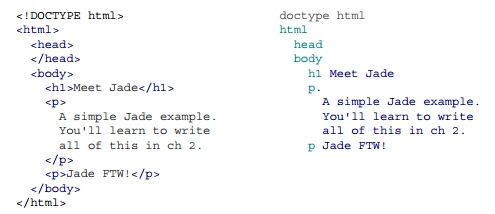
\includegraphics[width=0.7\textwidth]{./Pictures/jade.jpg}
  \rule{0.7\textwidth}{1pt}
 \caption{Jade example}
  \label{fig:jade}
\end{figure}


Both of the preceding code examples mean the exact same thing, except one is
much shorter. This is Jade, a powerful, terse templating language that is compiled
into HTML. In addition to the syntactical improvements, Jade lets you simplify
redundant markup with programmed logic. Also, it allows you to create templates
that can take in and display data.\cite{2}

\subparagraph*{Why should I preprocess?}
\hfill \break
Jade really is just one option in a whole class of preprocessors. To have a complete
understanding of Jade, we should understand why this class of languages was created.\cite{2}


Preprocessors are high-level languages that offer syntactical and functional
improvements over their "vanilla" (non-preprocessed) counterparts. These high-level
languages allow you to write the markup in a better language that is compiled down
to normal (vanilla) HTML. Thus, they are there purely to improve your productivity,
without affecting their compatibility with existing technologies.\cite{2}


Preprocessing, in general, offers many benefits over writing vanilla HTML. Standard
Generalized Markup Language (SGML), the predecessor of HTML, was created to
be robust and easy to parse at the expense of being clean and easy to write. Because
of this, a variety of preprocessors have emerged that offer a more terse syntax.\cite{2}


Occasionally, people will avoid preprocessing because it adds another step, that is,
another layer of abstraction to the end result. However, improvements in code
readability and ease of writing far outweigh the inconvenience of this additional
step. Furthermore, anything more complex than a static site will require a "build"
step anyway, to inject whatever dynamic content the site has.\cite{2}

\subparagraph*{How Jade preprocesses}
\hfill \break
In the case of Jade, this preprocessing is done by compiling templates into JS and
then rendering them to HTML, as shown in the following diagram:(Figure \ref{fig:jade_diagram})
\begin{figure}[h!]
  \centering
    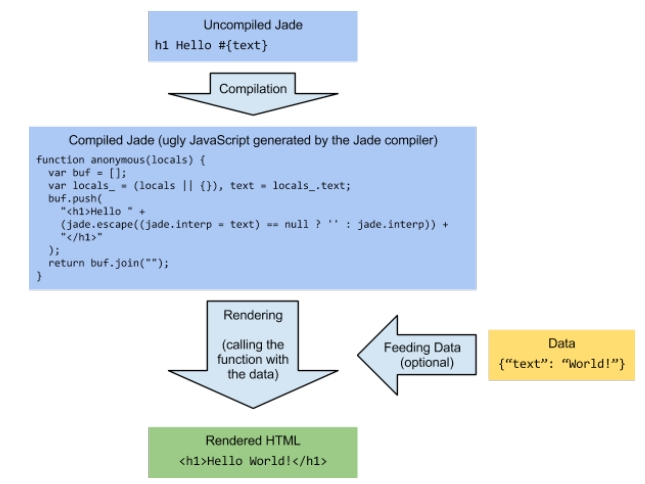
\includegraphics[width=1\textwidth]{./Pictures/jade_diagram.jpg}
  \rule{1\textwidth}{1pt}
 \caption{Jade example}
  \label{fig:jade_diagram}
\end{figure}

Because Jade's compiled templates really are just JavaScript functions that output
HTML, they can be rendered on both the server and in the browser.\cite{2}
\subsubsection{CSS (Cascading Style Sheets)}
Cascading Style Sheets (CSS) is a style sheet language used for describing the look and formatting of a document written in a markup language. While most often used to change the style of web pages and user interfaces written in HTML and XHTML, the language can be applied to any kind of XML document, including plain XML, SVG and XUL. Along with HTML and JavaScript, CSS is a cornerstone technology used by most websites to create visually engaging webpages, user interfaces for web applications, and user interfaces for many mobile applications.\cite{22}


CSS is designed primarily to enable the separation of document content from document presentation, including elements such as the layout, colors, and fonts. This separation can improve content accessibility, provide more flexibility and control in the specification of presentation characteristics, enable multiple HTML pages to share formatting by specifying the relevant CSS in a separate .css file, and reduce complexity and repetition in the structural content, such as semantically insignificant tables that were widely used to format pages before consistent CSS rendering was available in all major browsers. CSS makes it possible to separate presentation instructions from the HTML content in a separate file or style section of the HTML file. For each matching HTML element, it provides a list of formatting instructions. For example, a CSS rule might specify that "all heading 1 elements should be bold," leaving pure semantic HTML markup that asserts "this text is a level 1 heading" without formatting code such as a <bold> tag indicating how such text should be displayed.\cite{22}


This separation of formatting and content makes it possible to present the same markup page in different styles for different rendering methods, such as on-screen, in print, by voice (when read out by a speech-based browser or screen reader) and on Braille-based, tactile devices. It can also be used to display the web page differently depending on the screen size or device on which it is being viewed. While the author of a web page typically links to a CSS file within the markup file, readers can specify a different style sheet, such as a CSS file stored on their own computer, to override the one the author has specified. If the author or the reader did not link the document to a style sheet, the default style of the browser will be applied. Another advantage of CSS is that aesthetic changes to the graphic design of a document (or hundreds of documents) can be applied quickly and easily, by editing a few lines in one file, rather than by a laborious (and thus expensive) process of crawling over every document line by line, changing markup.\cite{22}


The CSS specification describes a priority scheme to determine which style rules apply if more than one rule matches against a particular element. In this so-called cascade, priorities or weights are calculated and assigned to rules, so that the results are predictable.
The CSS specifications are maintained by the World Wide Web Consortium (W3C). Internet media type (MIME type) text/css is registered for use with CSS by RFC 2318 (March 1998). The W3C operates a free CSS validation service for CSS documents.\cite{22}

\subsubsection{Less (stylesheet language)}
Less (sometimes stylized as LESS) is a dynamic stylesheet language that can be compiled into Cascading Style Sheets (CSS), or can run on the client-side and server-side. Designed by Alexis Sellier, Less is influenced by Sass and has influenced the newer "SCSS" syntax of Sass, which adapted its CSS-like block formatting syntax. Less is open-source. Its first version was written in Ruby, however in the later versions, use of Ruby has been deprecated and replaced by JavaScript. The indented syntax of Less is a nested metalanguage, as valid CSS is valid Less code with the same semantics. Less provides the following mechanisms: variables, nesting, mixins, operators and functions; the main difference between Less and other CSS precompilers being that Less allows real-time compilation via less.js by the browser.\cite{23}
%\subsubsection{CoffeeScript}
\subsubsection{jQuery}
jQuery is a cross-platform JavaScript library designed to simplify the client-side scripting of HTML. jQuery is the most popular JavaScript library in use today. jQuery is free, open-source software licensed under the MIT License.
jQuery's syntax is designed to make it easier to navigate a document, select DOM elements, create animations, handle events, and develop Ajax applications. jQuery also provides capabilities for developers to create plug-ins on top of the JavaScript library. This enables developers to create abstractions for low-level interaction and animation, advanced effects and high-level, theme-able widgets. The modular approach to the jQuery library allows the creation of powerful dynamic web pages and web applications.
The set of jQuery core features—DOM element selections, traversal and manipulation—enabled by its selector engine (named "Sizzle" from v1.3), created a new "programming style", fusing algorithms and DOM data structures. This style influenced the architecture of other JavaScript frameworks like YUI v3 and Dojo, later stimulating the creation of the standard Selectors API.
Microsoft and Nokia bundle jQuery on their platforms. Microsoft includes it with Visual Studio for use within Microsoft's ASP.NET AJAX framework and ASP.NET MVC Framework while Nokia has integrated it into the Web Run-Time widget development platform. jQuery has also been used in MediaWiki since version 1.16.\cite{24}
\subsection{Tools Used for Developing}
\subsubsection{Sublime Text 2}
\subparagraph*{So, what is Sublime Text 2?}
\hfill \break
Sublime Text 2 (Figure \ref{fig:sublime}) is the latest version of the popular text editor Sublime Text. It is a full-featured text
editor great for editing local text files. It has many built-in features to aid in editing code, such as
syntax highlighting, auto-indenting, file type recognition, a handy file/folder sidebar for easily
editing of multiple files within a directory, macros to automate repetitious tasks, and tabs and a
split-window option to view and edit multiple files at the same time. With Sublime Text 2's plethora
of programmer-centric features, utilizing this editor can increase your productivity without
bogging you down like full-fledged \textbf{Integrated Development Environments (IDE)} such as \textit{Visual
Studio} and \textit{Eclipse}. \cite{3}
\begin{figure}[h!]
  \centering
    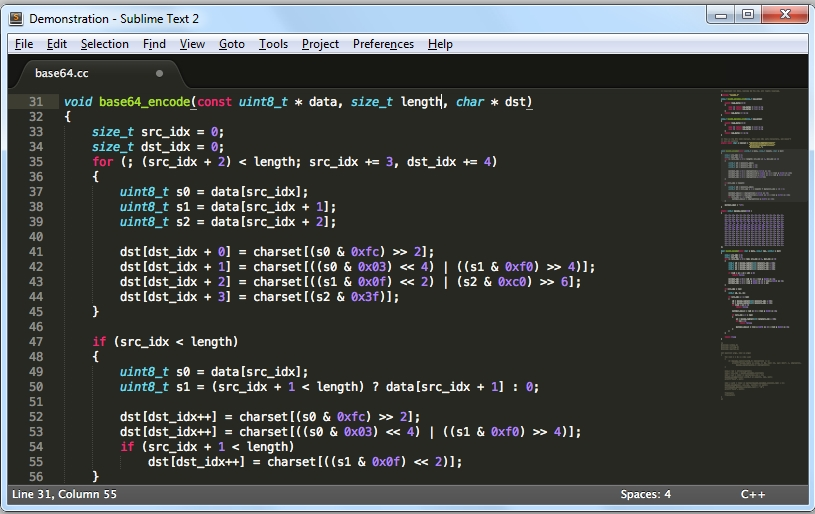
\includegraphics[width=1\textwidth]{./Pictures/sublime.jpg}
  \rule{1\textwidth}{1pt}
  \caption{Sublime Text 2}
    \label{fig:sublime}
\end{figure}

These IDEs certainly have their place, but the simplicity of Sublime Text 2
can be preferable in other scenarios. In addition to the many useful built-in features, Sublime Text
2 was built from the ground up to be extensible and the Sublime Text community has taken note
of it. Already, there are many useful extensions including interfaces for version control systems
such as git, snippet packages for jQuery and PHP, and syntax highlighting for popular CSS wrapper
languages such as LESS and SASS. Furthermore, the community has created Package Manager to
make discovering, installing, updating, and managing these plugins as simple as typing a hotkey
and a few characters. With a strong, configurable feature set and the ability to effortlessly extend
Sublime Text 2, it can truly become your text editor and increase your productivity in the same way
your tools should, while staying out of your way.\cite{3}




\subsubsection{GruntJs}
Over the recent years, the open source community has come up with great tools that
have eased development, such as CSS preprocessors, simple-to-use testing libraries,
and minification/compression libraries. Aimed to facilitate the automation of tasks,
Grunt helps both developers and sysadmins by speeding up the development time
and easing the production integration process.
This chapter will reintroduce you to Grunt and demonstrate the importance
of various other software tools. As you go further into the book, you will learn
how to develop your own projects using Grunt, with an increase in complexity
and applicability. In particular, you will acquire knowledge of how to use Grunt
efficiently as a software integration tool as well as learning about the best practices
surrounding web development today.\cite{6}
\subparagraph*{Introducing Grunt}
\hfill \break
Grunt is a simple-to-use task runner written with Node.js, a scalable JavaScript
software platform. A task runner is defined as a software tool used to automate
predefined tasks to ease the development and integration of large-scale projects
that are in production.\cite{6}

Grunt is currently used by large organizations such as Twitter and Adobe, and by
technologies such as jQuery. Through consistent updates, it has recently become
one of the most stable automation tools since its creation. The open source
community has embraced its simplicity compared to alternatives such as Ant or
Maven. Lastly, it is praised for its use of the ubiquitous language, JavaScript, thereby
easing the training among development teams. In this book, Grunt will be used to
automate the compilation of Sass to CSS and CoffeeScript to JavaScript. Minification
will be used to optimize page load times. Obfuscation, the mangling of information,
will also be automated to deter code theft and manipulation from the client side.
Grunt will be used to automate testing via the Mocha engine.
So, why should you use Grunt? In today's world of modern web applications, you
may find yourself using various tools that require compilation or preprocessing.
Likewise, you may wish to obfuscate code and minimize the size of your public files
in order to optimize the load time of our website. At other times, you could manually
call executables to perform these tasks. This would only waste more time that
would otherwise have been spent in the development of your app. With a simple,
customizable configuration file, Grunt allows you to set up a build script to automate
these activities via its community-curated plugins.\cite{6}
\subsubsection{PuTTY}
PuTTY  is a free and open-source terminal emulator, serial console and network file transfer application. It supports several network protocols, including SCP, SSH, Telnet, rlogin, and raw socket connection. It can also connect to a serial port (since version 0.59). The name "PuTTY" has no definitive meaning.
PuTTY was originally written for Microsoft Windows, but it has been ported to various other operating systems. Official ports are available for some Unix-like platforms, with work-in-progress ports to Classic Mac OS and Mac OS X, and unofficial ports have been contributed to platforms such as Symbian and Windows Mobile.
PuTTY was written and is maintained primarily by Simon Tatham and is currently beta software.\cite{19}
\begin{figure}[h!]
  \centering
  \vspace{-0.2cm}
    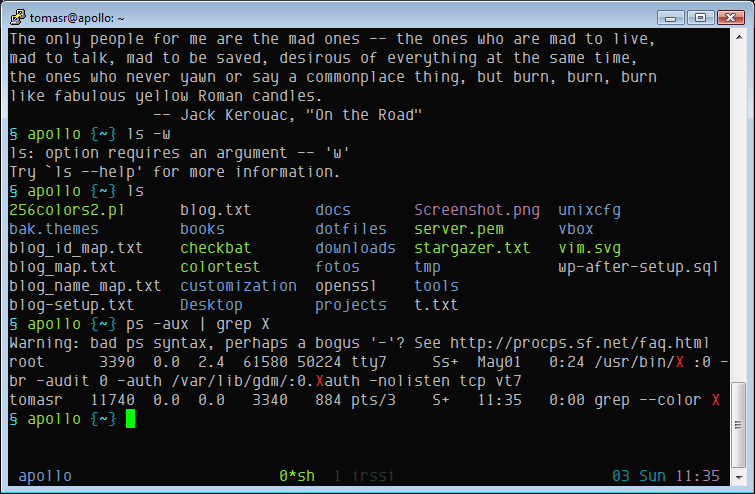
\includegraphics[width=1\textwidth]{./Pictures/putty_tango.png}
  \rule{1\textwidth}{1pt}
 \caption{Putty interface}
\end{figure}
